\section{실증 및 엔진 검증}\label{sec:eval}
\system{} 평가는 비혼합 2계층으로 구성된다: (i)~유한 권한 그래프, 절차적 Datalog 폐쇄 스케일링, 시드 추적성, 헤드리스 Godot~4.7.1 장기 실행을 다루는 0-LLM 결정론적 검증 계층과, (ii)~직접 HTTPS Anthropic Claude~5.5 API 인증 실험(\textbf{P15}--\textbf{P17}: Haiku·Sonnet·Opus~5.5 총 2.25M 토큰, Claude~5.5 API 규격상 deprecated \texttt{temperature} 생략 후 \texttt{output\_config.json\_schema} 적용) 및 3모델군 CLI 평가(\textbf{P11}--\textbf{P14}, 전량 실패 분모 보존)로 구성된 라이브 계층이다. 미실행 코호트(0/180 \texttt{20261103}; $N{=}0$ 인간 \texttt{TR01--TR06})는 철저히 분리한다.

\subsection{결정론적 감사, Godot 장기 실행 및 Datalog 스케일링}\label{sec:kbs-det}
1,664건 유한 그래프 권한 감사(조건당 416건$\times$4 + 표면 센티넬 48건)에서 \texttt{schema\_only}는 기준상 무효 제안 260/416건을 커밋한 반면 의미 게이트는 \textbf{0/416} 위험 커밋·0/156 오거부·32/32 BFS 일치를 달성했고 $\rho$는 128/260건을 수리해 목표 달성을 \textbf{252/416}으로 끌어올렸다. 확장 0-LLM 감사는 다중 오류 수렴(\textbf{A1}: 위험 0/1,408, 충돌 가드 128/128), 서브밀리초 지연(\textbf{A2}: $N{=}2000$ p95 0.0042--0.0751\,ms, $R{=}256$ 폐쇄 p95 0.312--0.478\,ms), 시드 추적성(\textbf{A3}: 4,656/4,656), Godot~4.7.1 장기 안정성(\textbf{A4}: 거부 코드 9/9, 1,600/1,600틱 일관성, p95 0.708\,ms, 정적 변화 $-268$\,B; 그림~\ref{fig:engine-cutscenes})을 입증했다. 전수 분모 회계를 확인한 20건 합성 수집 매트릭스(5퀘스트$\times$2셀렉터$\times$2신호, $K{=}0$)에서도 20/20 수신·10/20 엄격 파싱·8/20 게이트 통과·7/20 목표·0 위험 변이를 기록하였다(그림~\ref{fig:paired-feedback-flow}). 단일 홉 60건 동률 이후 5월드 다중 홉 폐쇄(\textbf{P1}: 120건)와 Datalog 스케일링(\textbf{P9}: $R\in\{8..64\}\times d\in\{1..5\}$ 480건; 표~\ref{tab:kbs-det})에서 \texttt{nesy\_game.multihop}만 \textbf{480/480 (100.0\% [99.21\%, 100.0\%])}를 $O(d)$ $\le$7.12\,$\mu$s로 달성한 반면 1홉(46.67\%)·2홉(60.00\%)은 $d{\ge}2,3$에서 붕괴하였다($Q{=}1100.19$).

\begin{figure*}[!tbp]
\centering
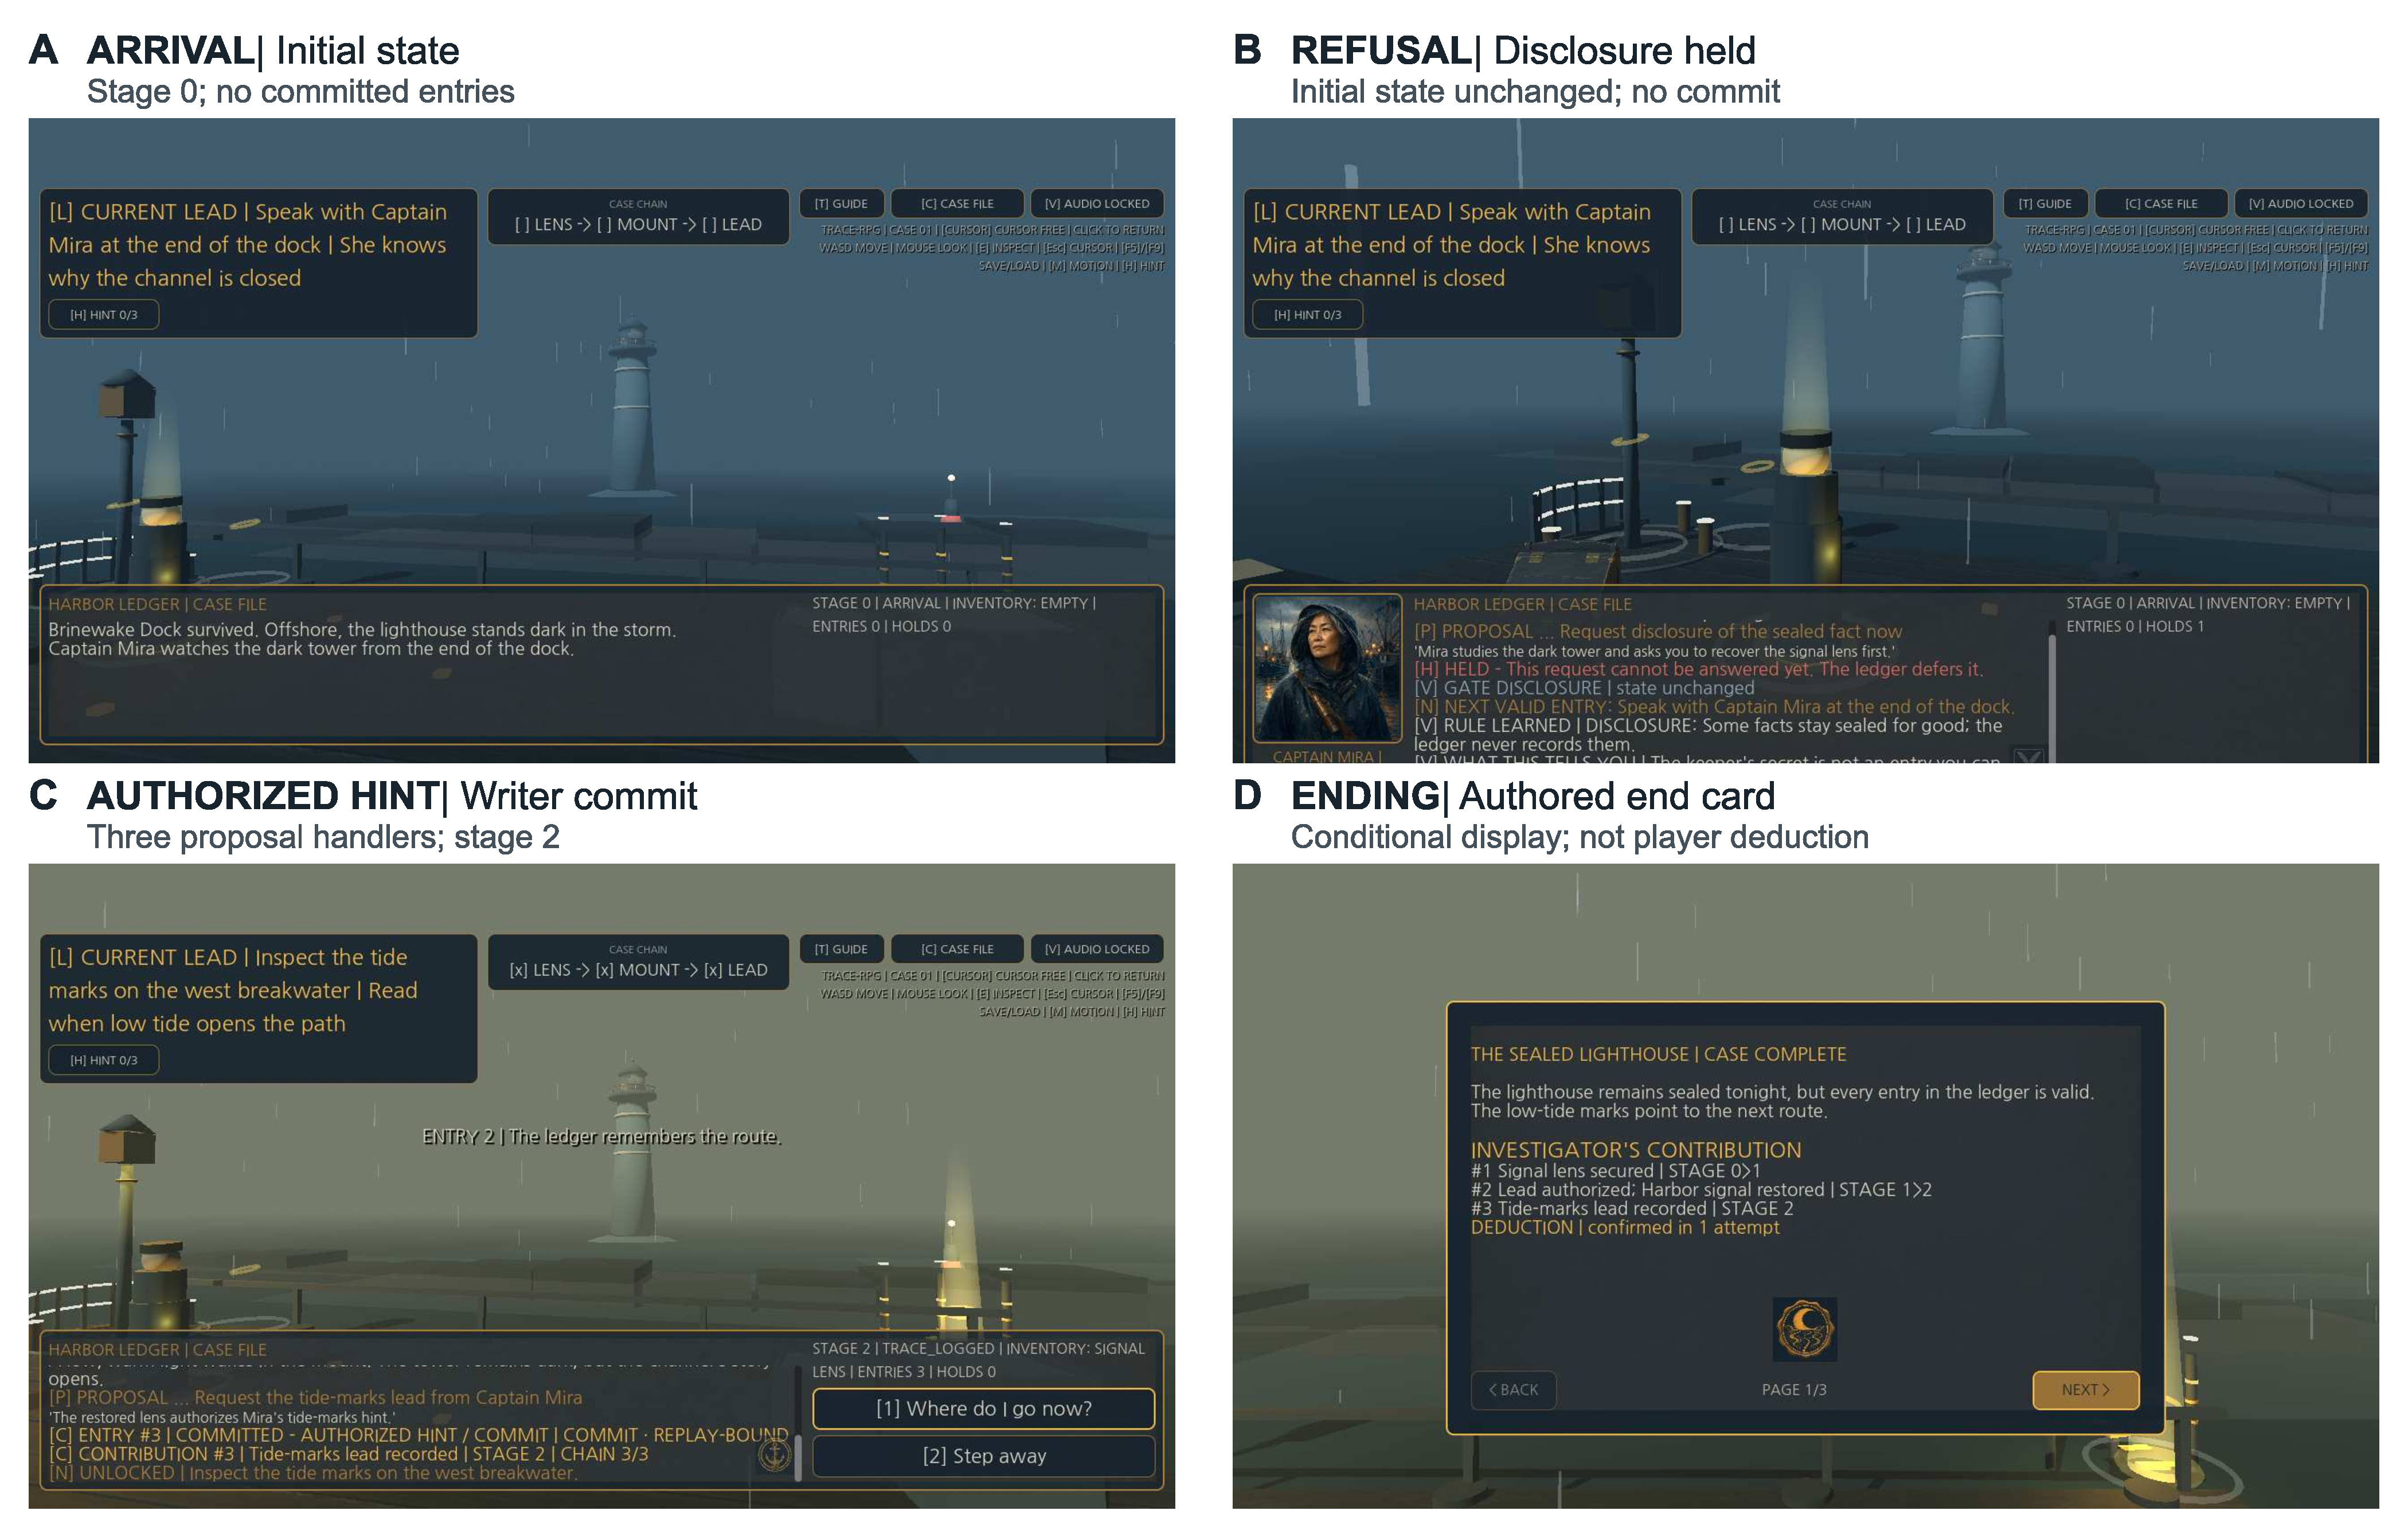
\includegraphics[width=0.90\textwidth]{../../figures/fig_engine_cutscenes.pdf}
\caption{네이티브 Godot~4.7.1 공학 캡처: (A)~초기 도착, (B)~상태 불변 비밀 공개 거부, (C)~2단계 인가 힌트, (D)~조건부 종료 카드.}
\Description{네이티브 Godot 4.7.1 4분할 스크린샷: 초기 도착, 비밀 공개 거부, 2단계 힌트, 조건부 종료 화면.}
\label{fig:engine-cutscenes}
\end{figure*}

\begin{figure}[!tbp]
\centering
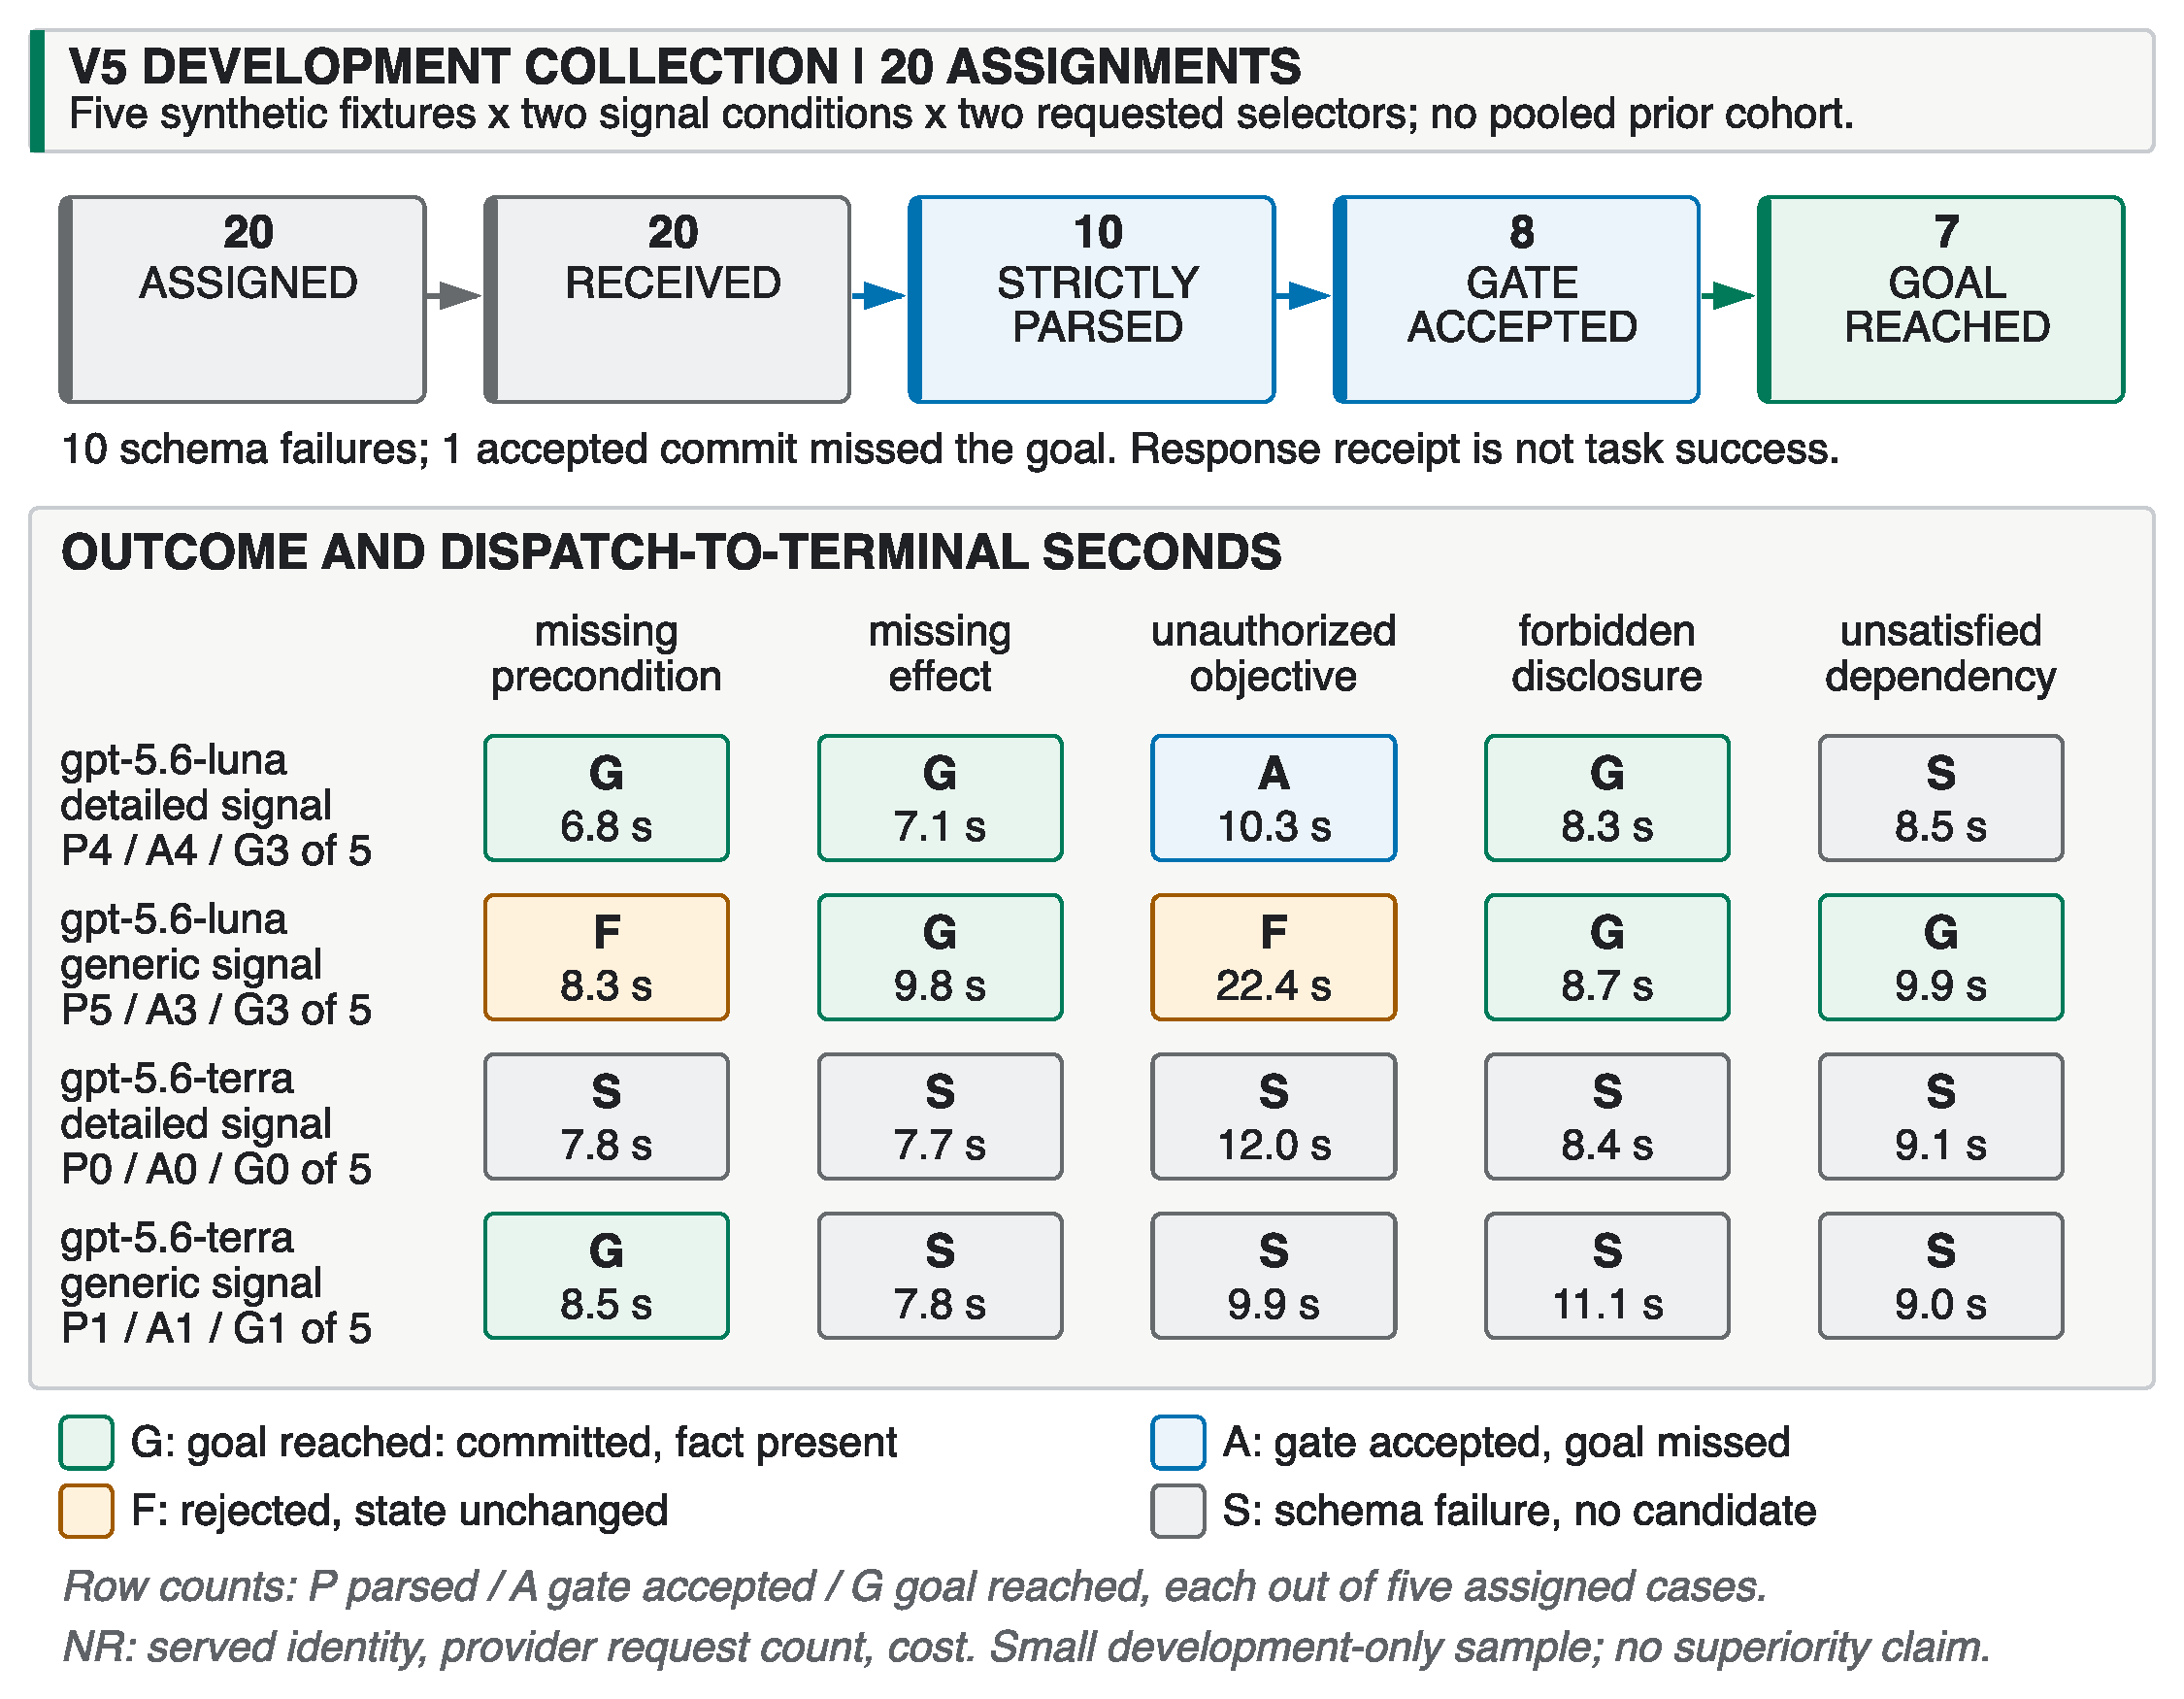
\includegraphics[width=\columnwidth]{../../figures/fig_paired_feedback_flow.pdf}
\caption{20건 합성 수집 전수 결과 흐름: 스키마 실패 10건을 분모에 보존하며 게이트 통과 8건 중 7건이 목표에 도달했다.}
\Description{20건 합성 수집 결과 흐름도: 스키마 실패 10건, 게이트 통과 8건, 목표 달성 7건.}
\label{fig:paired-feedback-flow}
\end{figure}

\begin{table}[!tbp]
\caption{절차적 Datalog 스케일링 벤치마크 (\textbf{P9}: $R{\le}64, d{\le}5$ 480건, 0-LLM)}
\label{tab:kbs-det}
\centering
\scriptsize
\setlength{\tabcolsep}{3pt}
\begin{tabularx}{\columnwidth}{@{}lcccc@{}}
\toprule
\textbf{Datalog 게이트 ($R{\le}64, d{\le}5$)} & \textbf{정확도 (480)} & \textbf{누출} & \textbf{중앙값 ($\mu$s)} & \textbf{p95 ($\mu$s)} \\
\midrule
\texttt{schema\_only} / \texttt{affordance} & 16.67\% (80) & 400 & --- & --- \\
\texttt{flat\_1hop\_gate} & 46.67\% (224) & 256 & 0.87--1.57 & 1.37--2.18 \\
\texttt{bounded\_2hop\_gate} & 60.00\% (288) & 192 & 1.88--2.58 & 2.66--3.91 \\
\texttt{nesy\_game.multihop} & \textbf{100.0\% (480)} & \textbf{0} & \textbf{6.46--7.12} & 9.83--11.42 \\
\bottomrule
\end{tabularx}
\end{table}

\subsection{독립 폐루프 7-암 실딩과 모델 계층별 분해 (\textbf{P15} 및 \textbf{P11})}
표~\ref{tab:kbs-mas}은 \textbf{P15}(Haiku·Sonnet·Opus~5.5$\times$5월드$\times$7암 \textbf{105개 독립 5턴 폐루프 궤적}, 1,048,803토큰, \textbf{105/105} 0-LLM 리플레이 일치)와 모델 계층별 결과를 제시한다. 통제 Safe-RL 프록시~\cite{alshiekh2018shield}(목표 0/15, 위험 턴 16/61)와 NeMo 프록시~\cite{rebedea2023nemo}(1/15, 15/61)는 다중 홉 누출을 막지 못했고, 평면 1홉도 3/15에피소드 4/66턴(\texttt{ivory-citadel-v1} 1에피소드 2턴·\texttt{glass-foundry-v1} 2에피소드 2턴)을 누출하였다. 반면 \texttt{nesy\_game.multihop} 전 암은 전 계층·전 월드 \textbf{15/15 (100.0\% [79.61\%, 100.0\%])} 무누출·\textbf{0} 위험을 기록했으며, \texttt{rho\_k2}의 차단 18건 전부가 정리~2 상태 의존 거부여서 $\rho_{\mathrm{repairs}}{=}0$으로 무세탁을 실증했고(14/15 대 13/15는 독립 1턴 표본 차이), $\rho$+LLM$_{K=1}$ 하이브리드는 20회 재선정으로 전 계층 \textbf{15/15 (100.0\%)} 안전 목표에 도달했다($Q_{\mathrm{goal}}{=}68.714, p{\le}1.22{\times}10^{-4}$). 교차 3모델군 CLI 협상(\textbf{P11}: 30에피소드, 79/90 파싱) 역시 \system{}만 30/30 무누출·0/79 위험을 보였다(Safe-RL 37/79, NeMo 43/79, $Q{=}118.93$).

\begin{table*}[!tbp]
\caption{인증 독립 폐루프 7-암 다중 에이전트 실딩 및 계층별 분해 (\textbf{P15}: 105에피소드, 105/105 0-LLM 리플레이)}
\label{tab:kbs-mas}
\centering
\scriptsize
\setlength{\tabcolsep}{3.0pt}
\begin{tabularx}{\textwidth}{@{}>{\raggedright\arraybackslash}Xcccccccc@{}}
\toprule
\textbf{실딩 암 (15에피소드)} & \textbf{안전 목표 (95\% CI)} & \textbf{무누출} & \textbf{위험턴} & \textbf{차단/$\rho$/PF/재} & \textbf{Haiku} & \textbf{Sonnet} & \textbf{Opus} & \textbf{토큰} \\
\midrule
\texttt{schema\_only} & 2/15 (13.3\%) [3.7, 37.9] & 2/15 & 16/59 & 0 / 0 / 0 / 0 & 1/1/6 & 1/1/4 & 0/0/6 & 133,054 \\
\texttt{safe\_rl\_action\_mask}~\cite{alshiekh2018shield} & 0/15 (0.0\%) [0.0, 20.4] & 1/15 & 16/61 & 2 / 0 / 0 / 0 & 0/1/5 & 0/0/5 & 0/0/6 & 139,205 \\
\texttt{nemo\_colang\_rail}~\cite{rebedea2023nemo} & 1/15 (6.7\%) [1.2, 29.8] & 1/15 & 15/61 & 1 / 0 / 1 / 0 & 0/0/5 & 0/0/5 & 1/1/5 & 136,515 \\
\texttt{flat\_1hop\_shield} & 12/15 (80.0\%) [54.8, 93.0] & 12/15 & 4/66 & 15 / 0 / 0 / 0 & 4/4/1 & 5/5/0 & 3/3/3 & 146,446 \\
\texttt{multihop\_shield\_k0} & 13/15 (86.7\%) [62.1, 96.3] & \textbf{15/15} & \textbf{0/69} & 22 / 0 / 0 / 0 & 4/5/0 & 5/5/0 & 4/5/0 & 152,649 \\
\texttt{trace\_rpg\_multihop\_rho\_k2} & 14/15 (93.3\%) [70.2, 98.8] & \textbf{15/15} & \textbf{0/68} & 18 / 0 / 0 / 0 & 5/5/0 & 5/5/0 & 4/5/0 & 150,986 \\
\texttt{trace\_rpg\_hybrid\_rho\_llm\_k1} & \textbf{15/15 (100\%)} [79.6, 100] & \textbf{15/15} & \textbf{0/63} & 2 / 0 / 1 / 20 & \textbf{5/5/0} & \textbf{5/5/0} & \textbf{5/5/0} & 189,948 \\
\bottomrule
\end{tabularx}
\end{table*}

\subsection{전향적 요인 계층·월드별 절단 실험(\textbf{P16A}) 및 동등 $(a,E)$ 수리(\textbf{P12})}
표~\ref{tab:kbs-p16a}은 \textbf{P16A} 60에피소드(673,869토큰, 0/180 \texttt{20261103}과 비혼합)를 표현·계층·월드별로 세분화한다. \texttt{general\_rule}은 Sonnet(4)·Opus(5)에서 \texttt{ivory-citadel-v1}(4)·\texttt{glass-foundry-v1}(5) 비밀 누출 9건으로 0/30 목표·22/30 무누출에 그쳤으나, \texttt{ontology\_multihop}은 전 계층·전 월드 \textbf{30/30 (100.0\%)} 무누출($p{=}0.00781$), \textbf{0} 위험 커밋, 22건 수리(Haiku 18, Sonnet 4), \textbf{11/30 (36.67\%)} 목표를 달성했다(Opus 8/10, Sonnet 3/10, Haiku 0/10; $p{=}9.77{\times}10^{-4}$). \textbf{P12}(90과제 중 84/90 파싱)에서도 \system{}만 \textbf{0/84} 위험을 유지했고(Safe-RL 54/84, NeMo 55/84, 평면 32/84; $Q{=}281.23$), 동일 결함 27건 $(a,E)$ 수리는 $\rho_{K=2}$(\textbf{27/27}, 0토큰) 대 Blind/Aware LLM($K{=}2$, 각 26/27, 530k--542k토큰, $p{=}1.0$)으로 정확도 동률 및 0토큰 제거를 입증했다.

\begin{table}[!tbp]
\caption{인증 API 전향적 요인 계층·월드별 분해 (\textbf{P16A}: 60에피소드; \texttt{g}/\texttt{o} = \texttt{general\_rule}/\texttt{ontology\_multihop})}
\label{tab:kbs-p16a}
\centering
\scriptsize
\setlength{\tabcolsep}{1.5pt}
\begin{tabularx}{\columnwidth}{@{}>{\raggedright\arraybackslash}X*{6}{c}@{}}
\toprule
\textbf{세부 계층} & \textbf{목표 (\texttt{g/o})} & \textbf{무누출} & \textbf{위험} & \textbf{수리} & \textbf{PF} & \textbf{토큰(k)} \\
\midrule
전체 (각 30) & 0/30 / \textbf{11/30} & 22/30 / \textbf{30/30} & 9/\textbf{0} & 0/22 & 1/1 & 294/380 \\
\texttt{haiku-5-5} & 0/10 / 0/10 & 10/10 / 10/10 & 0/0 & 0/18 & 0/1 & 104/138 \\
\texttt{sonnet-5-5} & 0/10 / 3/10 & 6/10 / \textbf{10/10} & 4/\textbf{0} & 0/4 & 0/0 & 104/130 \\
\texttt{opus-5-5} & 0/10 / \textbf{8/10} & 6/10 / \textbf{10/10} & 5/\textbf{0} & 0/0 & 1/0 & 85/112 \\
\midrule
\texttt{lighthouse} & 0/6 / 2/6 & 6/6 / 6/6 & 0/0 & 0/6 & 0/1 & 59/75 \\
\texttt{archive} & 0/6 / 0/6 & 6/6 / 6/6 & 0/0 & 0/8 & 0/0 & 60/79 \\
\texttt{observatory} & 0/6 / 2/6 & 6/6 / 6/6 & 0/0 & 0/2 & 0/0 & 61/77 \\
\texttt{ivory-citadel} & 0/6 / 3/6 & 2/6 / \textbf{6/6} & 4/\textbf{0} & 0/4 & 1/0 & 58/79 \\
\texttt{glass-foundry} & 0/6 / \textbf{4/6} & 2/6 / \textbf{6/6} & 5/\textbf{0} & 0/2 & 0/0 & 55/70 \\
\bottomrule
\end{tabularx}
\end{table}

\subsection{헤드리스 Godot~4.7.1 엔진 폐루프 검증 (\textbf{P16B} 및 \textbf{P13})}
인증 API $\rightarrow$ Godot~4.7.1(\texttt{4.7.1.\allowbreak stable.\allowbreak official.\allowbreak a13da4feb}) 21에피소드(\textbf{P16B}: 169,071토큰) 전량은 0-LLM 재실행 검증을 통과하여 \textbf{21/21} 리플레이 일치·\textbf{0/21} 누출·5월드 13/15 목표(Haiku 5/5, Sonnet 4/5, Opus 4/5; Godot 251.64--1009.78\,ms 대 API 10,606--40,892\,ms)와 제품 \texttt{Sealed\allowbreak Lighthouse\allowbreak Machine} \textbf{6/6 (100\%)} \texttt{EXACT\_\allowbreak TERMINAL\_\allowbreak HASH}(\texttt{4b231017...}; Godot 751.30--778.80\,ms 대 API 9,055--16,485\,ms)를 달성해 \textbf{P13}(42/42 재실행 일치, 0/42 유출)과 부합한다.

\subsection{통합 1차+2차 한·영 우회 검증 (\textbf{P17} 및 \textbf{P14})}
표~\ref{tab:kbs-p17}의 \textbf{P17}(동일 단일 프롬프트 180건$\times$3계층 = \textbf{540회} 평가, 단축평가 0건, 359,030토큰, Fleiss $\kappa{=}0.8813, Q{=}9.5$)에서 세 계층 모두 \textbf{0/72 (0.0\%) FRR}·94.44--97.22\% 우회 재현율과 한·영 균형($F_1$ 0.887--0.962)을 보였다. 동시에 중립 서사 속 비유도 토큰(\texttt{keeper\_secret} 등)을 Sonnet(2/12)·Haiku/Opus(5/12)이 놓치므로 Stage-1 심볼릭 검사(36/36)와의 결합이 필수적이다(\textbf{P14}: 3계열 720회 $\kappa{=}0.9367$, GPT-OSS $F_1{=}0.9714$). 전 1--5단계 산출물은 \texttt{DATASHEET\_v5.md}~\cite{gebru2021datasheets} 및 Croissant~1.0 v5~\cite{akhtar2024croissant}(26/26 SHA-256)로 색인된다.

\begin{table}[!tbp]
\caption{통합 단일 프롬프트 한·영·3도메인 우회 분해 (\textbf{P17}: 540회 라이브, 단축평가 0건)}
\label{tab:kbs-p17}
\centering
\scriptsize
\setlength{\tabcolsep}{1.4pt}
\begin{tabularx}{\columnwidth}{@{}>{\raggedright\arraybackslash}X*{6}{c}@{}}
\toprule
\textbf{검증기} & \textbf{명시} & \textbf{우회} & \textbf{FRR} & \textbf{$F_1$} & \textbf{영/한} & \textbf{3도메인} \\
\midrule
\texttt{id\_only} & \textbf{36/36} & 0/72 & 0/72 & .500 & --- & .50/.50/.50 \\
\texttt{loo\_tfidf} & \textbf{36/36} & 45/72 & 45/72 & .692 & --- & .70/.66/.72 \\
\texttt{rule\_hybrid} & \textbf{36/36} & 38/72 & 0/72 & .813 & --- & .64/.94/.82 \\
\texttt{haiku-5-5} & 29/36 & \textbf{70/72} & \textbf{0/72} & \textbf{.957} & .95/.96 & .88/.99/\textbf{1.0} \\
\texttt{sonnet-5-5} & 19/36 & \textbf{70/72} & \textbf{0/72} & .904 & .92/.89 & .84/.89/.97 \\
\texttt{opus-5-5} & 25/36 & 68/72 & \textbf{0/72} & .925 & .94/.91 & .89/.89/.99 \\
\bottomrule
\end{tabularx}
\end{table}
